%!TEX program = pdflatex
\documentclass{standalone}
\usepackage[UTF8]{ctex}
\usepackage{caption}
\usepackage{amsmath}
\usepackage{tikz}
\usepackage{mathdots}
\usepackage{yhmath}
\usepackage{cancel}
\usepackage{color}
\usepackage{siunitx}
\usepackage{array}
\usepackage{multirow}
\usepackage{amssymb}
\usepackage{gensymb}
\usepackage{tabularx}
\usepackage{booktabs}
\usetikzlibrary{fadings}
\tikzset{every picture/.style={line width=0.75pt}} %set default line width to 0.75pt    

\begin{document}


\tikzset{every picture/.style={line width=0.75pt}} %set default line width to 0.75pt        

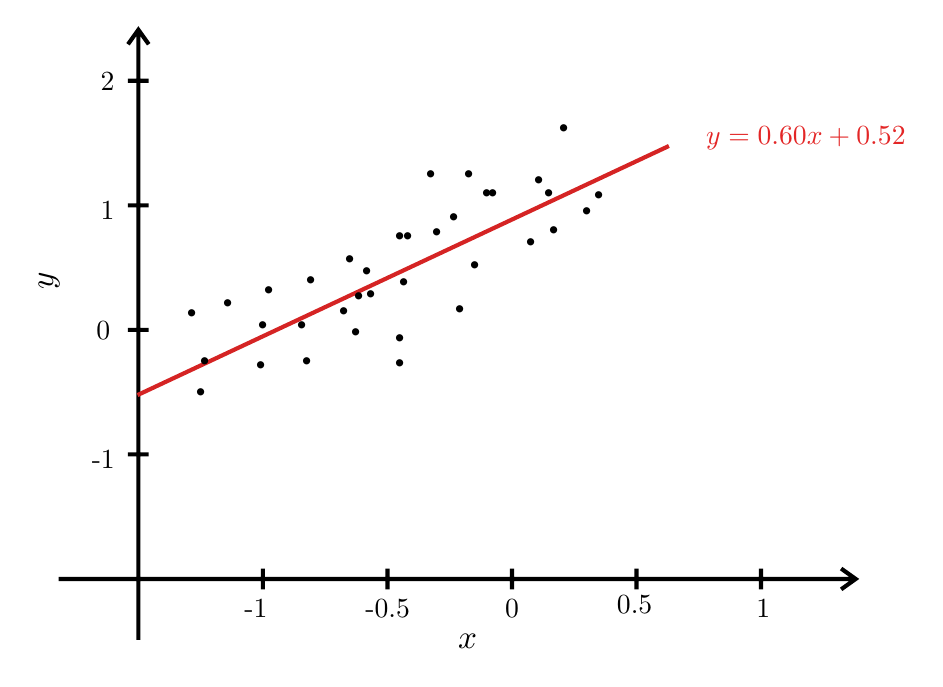
\begin{tikzpicture}[x=0.75pt,y=0.75pt,yscale=-1,xscale=1]
%uncomment if require: \path (0,635.1999969482422); %set diagram left start at 0, and has height of 635.1999969482422

%Shape: Axis 2D [id:dp27909638269830717] 
\draw [line width=1.5]  (180,484.6) -- (564,484.6)(218.4,220) -- (218.4,514) (557,479.6) -- (564,484.6) -- (557,489.6) (213.4,227) -- (218.4,220) -- (223.4,227) (278.4,479.6) -- (278.4,489.6)(338.4,479.6) -- (338.4,489.6)(398.4,479.6) -- (398.4,489.6)(458.4,479.6) -- (458.4,489.6)(518.4,479.6) -- (518.4,489.6)(213.4,424.6) -- (223.4,424.6)(213.4,364.6) -- (223.4,364.6)(213.4,304.6) -- (223.4,304.6)(213.4,244.6) -- (223.4,244.6) ;
\draw   ;
%Straight Lines [id:da8275794161745984] 
\draw [color={rgb, 255:red, 213; green, 36; blue, 36 }  ,draw opacity=1 ][fill={rgb, 255:red, 207; green, 33; blue, 33 }  ,fill opacity=1 ][line width=1.5]    (218,396) -- (474,276) ;



% Text Node
\draw (275,499) node  [align=left] {\mbox{-}1};
% Text Node
\draw (338.5,499) node  [align=left] {\mbox{-}0.5};
% Text Node
\draw (398.5,499) node  [align=left] {0};
% Text Node
\draw (457.5,497) node  [align=left] {0.5};
% Text Node
\draw (519.5,499) node  [align=left] {1};
% Text Node
\draw (201.5,427) node  [align=left] {\mbox{-}1};
% Text Node
\draw (201.5,365) node  [align=left] {0};
% Text Node
\draw (203.5,307) node  [align=left] {1};
% Text Node
\draw (203.5,245) node  [align=left] {2};
% Text Node
\draw (324.5,349.5) node [scale=2.488]  {$\mathbb{{\textstyle \cdot }}$};
% Text Node
\draw (344.5,369.5) node [scale=2.488]  {$\mathbb{{\textstyle \cdot }}$};
% Text Node
\draw (328.5,337.5) node [scale=2.488]  {$\mathbb{{\textstyle \cdot }}$};
% Text Node
\draw (330.5,348.5) node [scale=2.488]  {$\mathbb{{\textstyle \cdot }}$};
% Text Node
\draw (277.5,382.5) node [scale=2.488]  {$\mathbb{{\textstyle \cdot }}$};
% Text Node
\draw (389.5,299.5) node [scale=2.488]  {$\mathbb{{\textstyle \cdot }}$};
% Text Node
\draw (261.5,352.5) node [scale=2.488]  {$\mathbb{{\textstyle \cdot }}$};
% Text Node
\draw (301.5,341.5) node [scale=2.488]  {$\mathbb{{\textstyle \cdot }}$};
% Text Node
\draw (244.5,357.5) node [scale=2.488]  {$\mathbb{{\textstyle \cdot }}$};
% Text Node
\draw (248.5,395.5) node [scale=2.488]  {$\mathbb{{\textstyle \cdot }}$};
% Text Node
\draw (317.5,356.5) node [scale=2.488]  {$\mathbb{{\textstyle \cdot }}$};
% Text Node
\draw (344.5,320.5) node [scale=2.488]  {$\mathbb{{\textstyle \cdot }}$};
% Text Node
\draw (362.5,318.5) node [scale=2.488]  {$\mathbb{{\textstyle \cdot }}$};
% Text Node
\draw (370.5,311.5) node [scale=2.488]  {$\mathbb{{\textstyle \cdot }}$};
% Text Node
\draw (281.5,346.5) node [scale=2.488]  {$\mathbb{{\textstyle \cdot }}$};
% Text Node
\draw (416.5,299.5) node [scale=2.488]  {$\mathbb{{\textstyle \cdot }}$};
% Text Node
\draw (380.5,334.5) node [scale=2.488]  {$\mathbb{{\textstyle \cdot }}$};
% Text Node
\draw (278.5,363.5) node [scale=2.488]  {$\mathbb{{\textstyle \cdot }}$};
% Text Node
\draw (346.5,342.5) node [scale=2.488]  {$\mathbb{{\textstyle \cdot }}$};
% Text Node
\draw (407.5,323.5) node [scale=2.488]  {$\mathbb{{\textstyle \cdot }}$};
% Text Node
\draw (250.5,380.5) node [scale=2.488]  {$\mathbb{{\textstyle \cdot }}$};
% Text Node
\draw (297.5,363.5) node [scale=2.488]  {$\mathbb{{\textstyle \cdot }}$};
% Text Node
\draw (323.5,366.5) node [scale=2.488]  {$\mathbb{{\textstyle \cdot }}$};
% Text Node
\draw (373.5,355.5) node [scale=2.488]  {$\mathbb{{\textstyle \cdot }}$};
% Text Node
\draw (418.5,317.5) node [scale=2.488]  {$\mathbb{{\textstyle \cdot }}$};
% Text Node
\draw (359.5,290.5) node [scale=2.488]  {$\mathbb{{\textstyle \cdot }}$};
% Text Node
\draw (386.5,299.5) node [scale=2.488]  {$\mathbb{{\textstyle \cdot }}$};
% Text Node
\draw (299.5,380.5) node [scale=2.488]  {$\mathbb{{\textstyle \cdot }}$};
% Text Node
\draw (320.5,331.5) node [scale=2.488]  {$\mathbb{{\textstyle \cdot }}$};
% Text Node
\draw (348.5,320.5) node [scale=2.488]  {$\mathbb{{\textstyle \cdot }}$};
% Text Node
\draw (440.5,300.5) node [scale=2.488]  {$\mathbb{{\textstyle \cdot }}$};
% Text Node
\draw (411.5,293.5) node [scale=2.488]  {$\mathbb{{\textstyle \cdot }}$};
% Text Node
\draw (377.5,290.5) node [scale=2.488]  {$\mathbb{{\textstyle \cdot }}$};
% Text Node
\draw (423.5,268.5) node [scale=2.488]  {$\mathbb{{\textstyle \cdot }}$};
% Text Node
\draw (434.5,308.5) node [scale=2.488]  {$\mathbb{{\textstyle \cdot }}$};
% Text Node
\draw (540,272.5) node   {$\textcolor[rgb]{0.89,0.15,0.15}{y=0.60x+0.52}$};
% Text Node
\draw (377,514.5) node [scale=1.2]  {$x$};
% Text Node
\draw (344.5,381.5) node [scale=2.488]  {$\mathbb{{\textstyle \cdot }}$};
% Text Node
\draw (175.46,341.06) node [scale=1.2,rotate=-269.66]  {$y$};


\end{tikzpicture}

\end{document}
